\fancyfoot[RE,LO]{Autor: Julia Gartner}

\section {Mobile Applications} \label {MobileApplications}

\subsection {Einleitung} \label {MAEinleitung}

Eine Mobile Application, oft nur App genannt, ist Software, die auf mobilen Ger�ten verwendet werden kann. Solche Ger�te sind z.B. Smartphones, Tablets oder Smartwatches und haben meistens entweder Android oder iOS als Betriebssystem\cite{reg401}. Generell gibt es viele Anwendungen f�r mobile App wie Kommunikation, E-Commerce und Weiterbildung\cite{reg402}. In unserem Fall hat das Software Interface prim�r die Aufgabe, die mithilfe des EOGs gesammelten Daten f�r den User graphisch darzustellen. Sekund�r gibt es eine Weckerfunktion.

\subsection {Allgemeines zur Mobilapp-Entwicklung} \label {MAAllgemeines}

Wie bereits in Kapitel \ref{MAEinleitung} erw�hnt, sind die meistverbreiteten Betriebssysteme, die die Umgebung f�r Mobile Apps darstellen, iOS und Android mit einem Marktanteil von 99\% im Jahr 2018 in den USA. Mobile Apps f�r diese beiden Betriebssysteme werden jedoch nicht in der selben Sprache geschrieben. F�r Android kann in Java oder Kotlin geschrieben werden, w�hrend f�r iOS Objective-C oder Swift verwendet wird. Das ist in der Praxis oft nicht optimal, da eine Anwendung erstens in zwei verschiedenen Sprachen geschrieben werden muss und zweitens auch zwei verschiedene Anwendungen gewartet werden m�ssen\cite{reg403}. Eine L�sung f�r dieses Problem sind Hybrid Mobile App Development Frameworks. Mit diesen Frameworks k�nnen Apps in einer Sprache geschrieben werden und trotzdem auf verschiedenen Betriebssystemen laufen\cite{reg404}.\\

\begin{figure}[H]
	\centering
		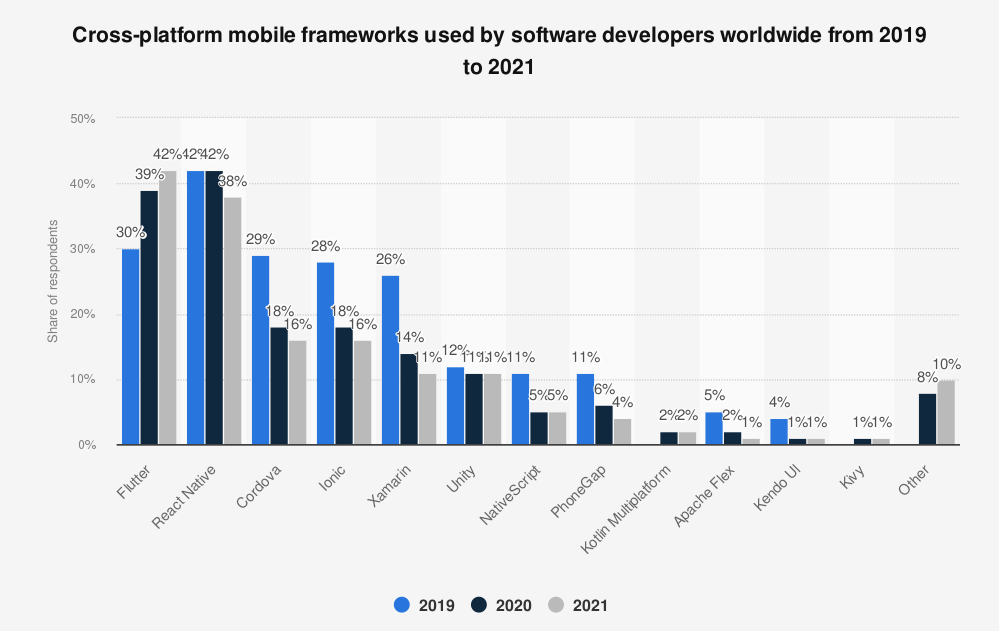
\includegraphics[width=0.9\textwidth]{Gartner/assets/cross_platform_use_statistic.png}
	\caption{Plattform�bergreifende Mobile-Frameworks die von Softwareentwicklern weltweit verwendet werden (2019 bis 2021)\cite{reg405}}
	\label{fig:cross_platform_use_statistic}
\end{figure}

Wie in Abbildung \ref{fig:cross_platform_use_statistic} zu sehen ist, sind die zwei meist verwendeten plattform�bergreifenden Mobile-Frameworks seit 2019 Flutter und React Native, was sich immer weiter absetzt. W�hrend im Jahr 2019 das meistverwendete Framwork noch React Native war, verwenden 2021 die meisten Entwickler bereits Flutter.  \\
React Native und Flutter unterscheiden sich in mehreren Hinsichten. Zum einen wird das React Native-Framework mit JavaScript verwendet, w�hrend ein Flutter-Projekt in Dart geschrieben wird. React Native erreicht die plattformunabh�ngige Anwendung durch eine Br�cke; ein React Native-Projekt in JavaScript auf einem Android-Ger�t z.B. kommuniziert �ber diese Br�cke mit nativen Komponenten des Betriebssystems. Bei Flutter hingegen wird ein Projekt beim Kompilieren von Dart direkt zu einer nativen Sprache �bersetzt, f�r ein Ger�t ist das also nicht zu unterscheiden von einer nativen App\cite{reg406}.

\subsubsection {Entwicklungsumgebung} \label{MAEntwicklungsemgebung}

VSCode, Android Studio Emulator

\subsection {Flussdiagramm} \label {MAFlussdiagramm}

\begin{figure}[H]
	\centering
		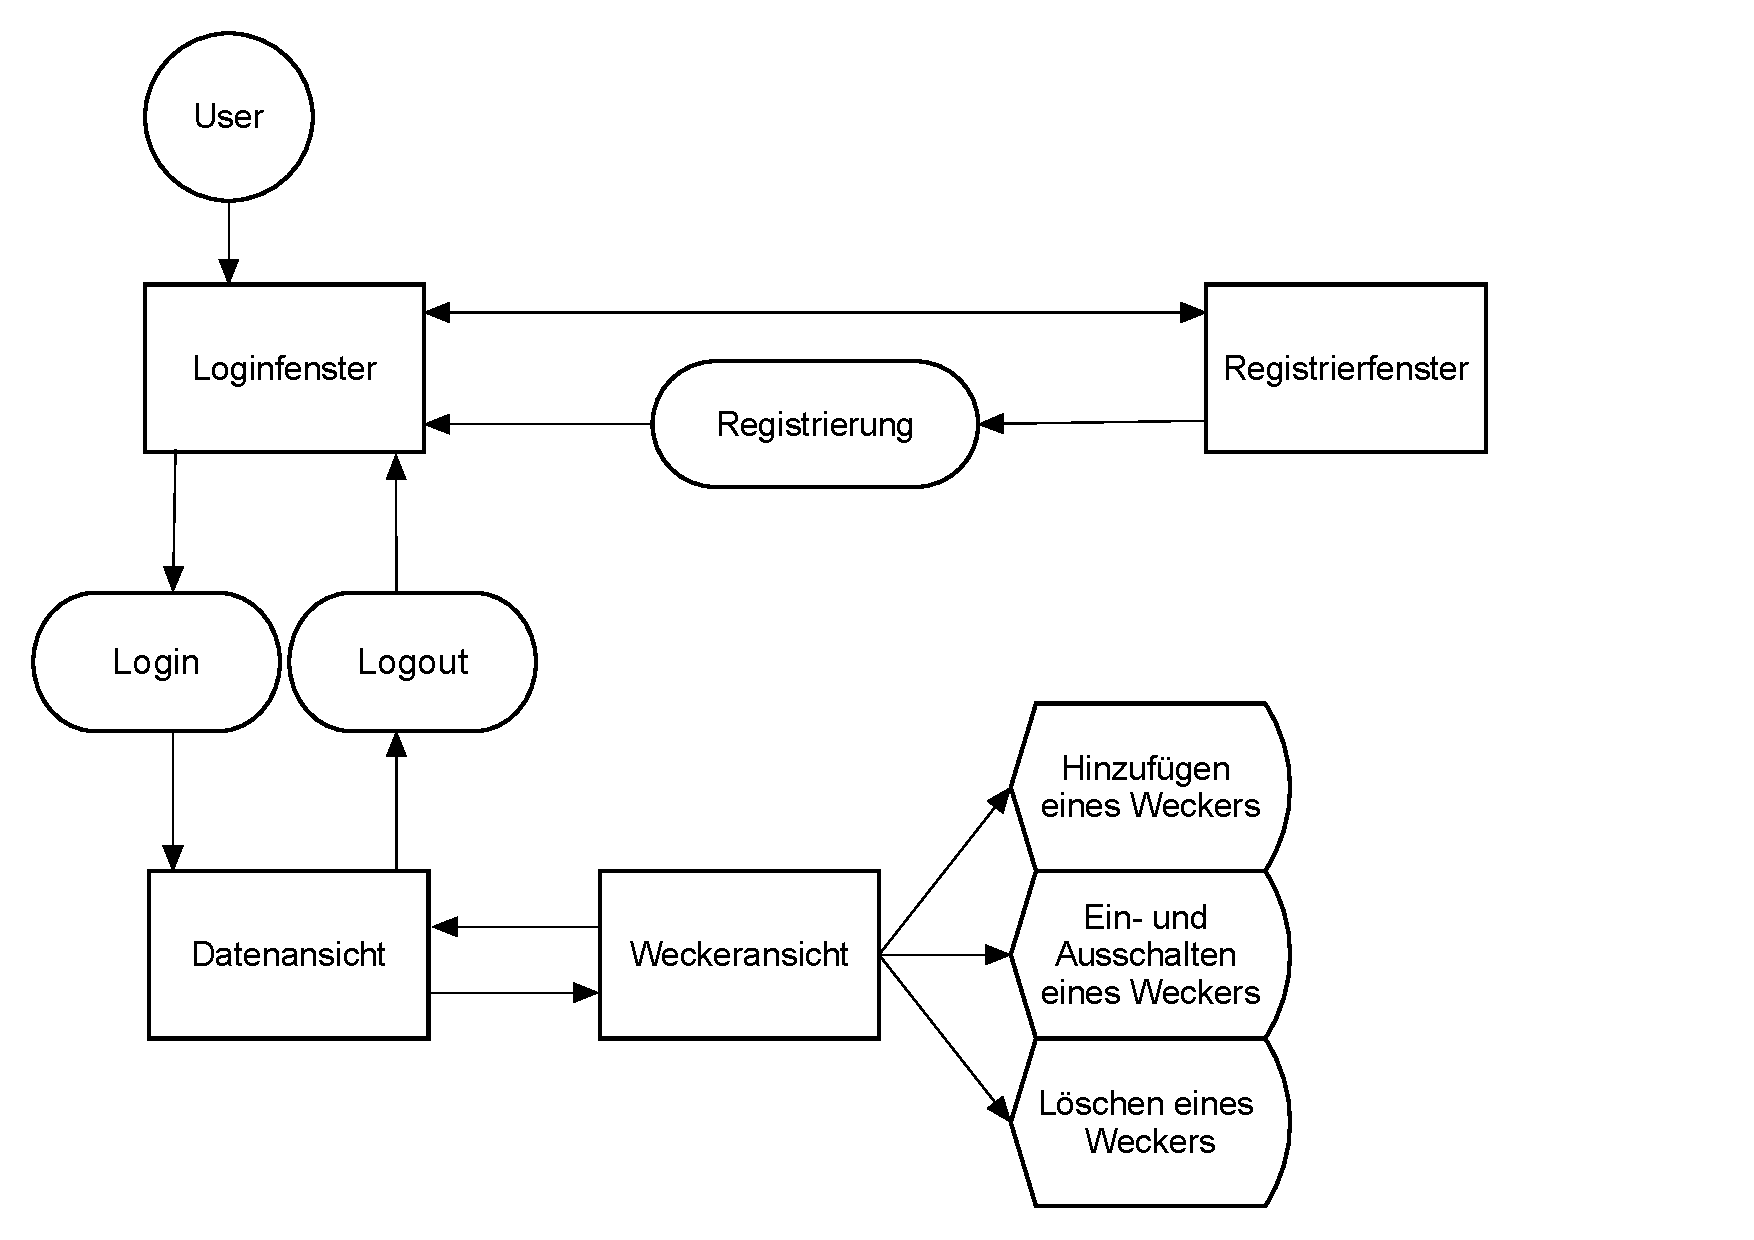
\includegraphics[width=0.9\textwidth]{Gartner/flussdiagramm.pdf}
	\caption{Flussdiagramm der Mobile Application}
	\label{fig:MA_Flussdiagramm}
\end{figure}

\begin{figure}[H]
	\centering
		
\includegraphics[width=0.45\textwidth]{Gartner/buffer.jpg}
	\caption{Loginfenster des GUI}
	\label{fig:MA_Loginfenster}
\end{figure}

\begin{figure}[H]
	\centering
		
\includegraphics[width=0.45\textwidth]{Gartner/buffer.jpg}
	\caption{Registrierfenster des GUI}
	\label{fig:MA_Registrierfenster}
\end{figure}

Der erste Bildschirm ist wie in Abbildung \ref{fig:MA_Flussdiagramm} zu erkennen entweder das Loginfenster oder der Homescreen mit der Datenansicht. Falls man die App zum ersten Mal �ffnet oder sich in der letzten Session abgemeldet hat, ist das in Abbildung \ref{fig:MA_Loginfenster} zu sehende Loginfenster der Startpunkt. Von hier aus kann sich der Benutzer entweder einloggen, wenn er schon einen Account hat, oder zum Registrierfenster, wie in Abbildung \ref{MA_Registrierfenster} gezeigt, wechseln, um sich zu registrieren. Wenn die Registrierung erfolgreich war, wird wieder zum Loginfenster geleitet. Es gibt aber auch die M�glichkeit, ohne Registrierung wieder zum Loginfenster zu wechseln. In beiden F�llen muss der Login im Loginfenster erfolgen, um die Datenansicht zu laden. \\

\begin{figure}[H]
	\centering
		
\includegraphics[width=0.45\textwidth]{Gartner/buffer.jpg}
	\caption{Datenansicht des GUI}
	\label{fig:MA_Datenansicht}
\end{figure}

Im Fall, dass der User sich bereits einmal eingeloggt und in der letzten Session nicht abgemeldet hat, wird direkt die Datenansicht geladen. Hier gibt es, wie in Abbildung \ref{MA_Datenansicht} zu sehen, eine Navigationsleiste am unteren Ende des Bildschirms, mit dem ausgew�hlt werden kann, ob die Daten- oder Weckeransicht gezeigt wird. \\
In der Datenansicht werden alle Messergebnisse der EOG-Messungen eines Benutzers angezeigt. Hier gibt es, abgesehen vom Scrollfeature, keine Interaktionsm�glichkeiten. \\

\begin{figure}[H]
	\centering
		
\includegraphics[width=0.45\textwidth]{Gartner/buffer.jpg}
	\caption{Weckeransicht des GUI}
	\label{fig:MA_Weckeransicht}
\end{figure}

Die Weckeransicht, gezeigt in Abbildung \ref{fig:MA_Weckeransicht}, erm�glicht eine Verwaltung der Weckerfunktion. M�gliche Interaktionen hier sind das Hinzuf�gen oder Entfernen und das Ein- oder Ausschalten eines Weckers. Hinzugef�gte Wecker werden ebenfalls hier angezeigt. \\

\begin{figure}[H]
	\centering
		
\includegraphics[width=0.45\textwidth]{Gartner/buffer.jpg}
	\caption{Logout des GUI}
	\label{fig:MA_Logout}
\end{figure}

Wie bereits in Abbildung \ref{MA_Datenansicht} und \ref{MA_Weckeransicht} zu erkennen, ist links oben in der Ansicht ein Menu Button implementiert. Das dahinterliegende Menu mit der Logout-Funktion ist in Abbildung \ref{MA_Logout} zu sehen. 

\subsection {Funktionalit�t} \label {}

\subsubsection {Framework} \label {MAFramework} 

Wie bereits in Kapitel \ref{MAEinleitung}

\subsubsection {Benutzerverwaltung} \label {}

\subsubsection {State-Management} \label{MAState}

Es gibt zwei verschiedne Arten von Widgets in Flutter: Stateless und Stateful Widgets. Stateful Widgets sind Widgets, die sich ver�ndern k�nnen, wenn z.B. Daten dargestellt werden oder der Benutzer mit dem Widget interagieren kann. Stateless Widgets hingegen sind Widgets, die sich nie ver�ndern\cite{reg407}.\\
State ist Information, die ermittelt werden kann, w�hrend ein Widget gebaut wird und sich auch �ndern kann. Beim Entwickeln einer App in Flutter muss also darauf geachtet werden, dass beim Auftreten solcher �nderungen ein Widget auch neu aufgebaut wird, da die dahinterliegenden Informationen sich sonst ge�ndert haben, aber nicht das Widget selbst. Das kann mit Methoden wie z.B. setState geregelt werden\cite{reg408}. Hier k�nnen aber Probleme entstehen, wenn State �ber verschiedene Klassen hinweg weitergegeben werden muss; Dies kann zwar mit �bergabeparametern gel�st werden, aber auch hier bleibt das genannte Problem bestehen und vor allem bei gr��eren Projekten ist die L�sung bei weitem nicht ideal.\\
Im Internet k�nnen viele Klassen gefunden werden, die State Management vereinfachen sollen. Eine der Basisklassen ist die InheritedWidget class. Die Logik hinter der Klasse ist, dass State im Baum nach unten vererbt werden kann, sich die verkn�pften Widgets sich bei einer �nderung des States in einem dar�berliegenden Widget also auch neu aufbauen\cite{reg409}. 
F�r das Projekt Sleepanalyzer wurde die Klasse provider zusammen mit ChangeNotifier verwendet, was einer der popul�rsten Ans�tze ist. Klassen k�nnen als ChangeNotifier Klasse angelegt werden. Andere Klassen k�nnen dann subscriben, um bei �nderungen verst�ndigt zu werden. Die Klasse Provider sorgt daf�r, dass State nicht durch den ganzen Widgetbaum weitergegeben werden muss, sondern direkt zu einem bestimmten Widget weitergegeben werde kann. Dazu muss allerdings eine Liste in einem Widget �ber einem Provider und dem Widget, in dem der State gebraucht wird angelegt sein\cite{410}.

\subsubsection {Permanenter Speicher} \label{}

\subsubsection {Data Fetching} \label{MADataFetching}

Da bei der Messung des EOGs die Daten direkt vom Mikrocontroller zu einem Server geschickt werden und dort auf einer Datenbank gespeichert werden, m�ssen diese zur Ansicht der Daten in der App zuerst vom Server angefragt werden. Wenn in der App zur Datenansicht gewechselt wird, entweder vom Loginfenster oder von der Weckeransicht, wird von einem Widget eine Funktion aufgerufen, in der ein Post-Request an den Server gestellt wird. Der body dieses Requests enth�lt die momentan g�ltige User-ID. Am Server werden alle Daten, die zu dieser ID vorhanden sind gesammelt und ebenfalls in einem Post-Request im JSON-Format zur�ckgesendet. Diese Daten werden dann in der App weiter verwertet. Im Folgenden werden alle einzelnen Schritte n�her erl�utert. 

\paragraph{Async functions} \label{MADataFetching_AsyncFunctions}

Da Vorg�nge wie das Warten auf eine Antwort des Servers nach dem Senden eines POST-Requests lange dauern, w�re es nicht gut, wenn alle anderen Vorg�nge w�hrenddessen blockiert sind. Deshalb gibt es Unterscheidungen zwischen synchronen und asynchronen Vorg�ngen. Bei synchronen Operationen wird ein Schritt nach dem anderen abgehandelt, w�hrend bei asynchronen Operationen w�hrenddessen andere Operationen durchgef�hrt werden k�nnen. Die Klasse, die f�r asynchrone Vorg�nge im Flutter-Framework verwendet wird ist die Future\flq T\frq{} Klasse. Ein \glqq future\grqq{} ist eine Instanz der Klasse Future und ist das Ergebniss einer asynchronen Funktion. Wenn nun eine asynchrone Funktion aufgerufen wird, wird ein unvollst�ndeiges future zur�ckgegeben. Dieses future wartet auf den wirklichen Wert, der von der Funktion zur�ckgegeben wird (falls eine Funktion einen R�ckgabewert hat). \\
Dies sorgt daf�r, dass w�hrend auf die Antwort des Servers gewartet werden muss, alle anderen Vorg�nge in der App weiter bestehen bleiben.

\paragraph{HTTP Requests} \label{}

Es gibt eine Reihe von Requests, die im HTTP-Protokoll angef�hrt sind und oft in zur Datenvermittelung verwendet werden. Zwei der h�ufigsten davon sind der POST- und der GET-Request. Diese beiden unterscheiden sich in mehreren Hinsichten. Wie der Name es annehmen l�sst ist ein GET-Request urspr�nglich f�r die Anfrage an einen Server nach Daten und ein POST-Request f�r das Vermitteln von Daten an den Server gedacht. Dies muss in der Praxis allerdings nicht immer eingehalten werden\cite{reg413}. \\
Einer der wichtigsten Unterschiede ist, dass bei einem GET-Request die gesamte Anfrage im Header eines Requests angef�hrt ist, und somit die L�nge auch an die maximale URL-L�nge eines Browsers angepasst werden muss; Ein GET-Request kann also f�r Internet Explorer zum Beispiel maximal 2.048 Zeichen, abz�glich der Anzahl der Zeichen des Pfads, betragen. \\
Bei einem POST-Request ist das nicht der Fall, da der Inhalt eines POST-Requests nicht im header, sondern im Message-body angef�hrt wird\cite{reg413},\cite{reg414}. \\

\paragraph {Implementierung} \label{MADataFetching_Implementierung}

\begin{figure}[H]
	\centering
		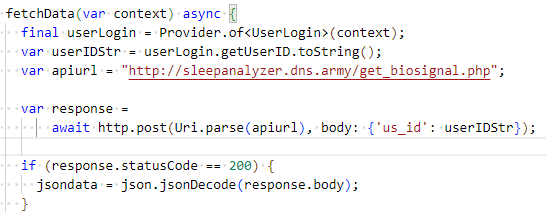
\includegraphics[width=0.9\textwidth]{Gartner/assets/async_post_json.png}
	\caption{Quellcodeausschnitt zur Kommunikation mit dem Server}
	\label{fig:async_post_json}
\end{figure}

In Abbildung \ref{fig:async_post_json} ist die Funktion zur Anfrage und Erhaltung der Daten vom Server zu sehen. Zuerst wird ein POST-Request geschickt, in dessen body die Benutzer-ID festgelegt ist. Die Antwort des Servers erfolgt im JSON-Format und muss dekodiert werden. 





\subsubsection {Graphische Darstellung der Daten} \label{}

syncfusion flutter charts

\subsubsection {Design} \label{}

Material Design






